\documentclass[11pt,a4paper]{article}
\usepackage[T1]{fontenc}
\usepackage[brazil]{babel}
\usepackage{lmodern,amsmath,graphicx,booktabs}
\usepackage[margin=2.4cm]{geometry}
\usepackage[hidelinks]{hyperref}
\graphicspath{{../results/}}

\title{Fidelidade visual com omissão de níveis na mistura Laplaciana de texturas}
\author{Icaro Vinicius \and Vinicius Macedo \and Caio Dias}
\date{Computação Gráfica --- IFNMG, 2026/2\\Versão preliminar}

\begin{document}
\maketitle

\begin{abstract}
Investigamos o efeito de agrupar bandas da mistura Laplaciana de texturas usando níveis alternados da cadeia de mipmaps. Comparamos uma interpolação linear por pixel, uma referência Laplaciana com seis bandas e uma variante que usa os níveis 0, 2, 4 e 6. Em quatro cenários offline com texturas de albedo, a variante obteve SSIM entre 0,999888 e 0,999999 e PSNR entre 52,25 e 77,12\,dB em relação à referência, na região de transição. A contagem teórica de amostras passa de 21 para 12 por fragmento. A medição de tempo em GPU faz parte da avaliação final.
\end{abstract}

\section{Introdução}
A interpolação de texturas é usada para combinar materiais em superfícies virtuais. Uma faixa estreita de interpolação pode gerar uma costura aparente, enquanto uma faixa larga pode suavizar detalhes na sobreposição. Wronski~\cite{wronski2025} usa mipmaps existentes para aproximar uma decomposição Laplaciana no shader, modulando a largura da transição de acordo com a frequência espacial. A questão deste trabalho é quanto a omissão de níveis altera a saída em relação à variante completa e quanto ela economiza em uma implementação GPU controlada.

\section{Trabalhos relacionados}
A mistura multirresolução de Burt e Adelson~\cite{burt1983} combina bandas de frequências com transições dependentes da escala. Wronski~\cite{wronski2025} aplica o princípio à mistura de texturas com mipmaps e apresenta a omissão de níveis na Seção 6.2. Nossa contribuição é avaliar essa otimização com entradas e métricas reproduzíveis e testar a relação entre fidelidade e custo em uma implementação WebGL.

\section{Método}
Sejam \(A_k\), \(B_k\) e \(M_k\) os mipmaps das duas texturas e da máscara, amostrados no mesmo ponto. A baseline é \(\operatorname{lerp}(A_0,B_0,M_0)\). Para uma sequência \(k_0,\ldots,k_s\), calculamos
\begin{equation}
  I = \sum_{i=0}^{s-1} \operatorname{lerp}(A_{k_i}-A_{k_{i+1}},
      B_{k_i}-B_{k_{i+1}}, M_{k_i}) + \operatorname{lerp}(A_{k_s},B_{k_s},M_{k_s}).
\end{equation}
A referência percorre \(0,1,\ldots,6\). A variante usa \(0,2,4,6\) e pesa cada banda agrupada pela máscara de seu nível mais fino. Ambos usam o mesmo residual no nível 6. No executor Python, cada mipmap é reduzido diretamente a partir da entrada de 8 bits e ampliado por interpolação bilinear. A demo WebGL usa viés de LOD e uma pirâmide de máscara em alvos separados. As métricas deste artigo foram calculadas no executor Python.

\section{Protocolo experimental}
Combinamos dois pares de texturas de albedo de \(1024\times1024\) pixels com duas máscaras, uma orgânica derivada de Perlin e uma rampa horizontal. A máscara orgânica é \(M_0=\operatorname{clamp}(8(P-0{,}55)+0{,}5,0,1)\). A região de interesse (ROI) contém os pixels com \(0{,}05<M_0<0{,}95\). Calculamos PSNR em RGB na ROI e SSIM médio por canal com janela gaussiana \(11\times11\) e \(\sigma=1{,}5\)~\cite{wang2004}. Para SSIM, cada centro pertence à ROI e a janela cabe na imagem. Medimos também a variância local média da luma em janelas \(7\times7\) centradas na ROI. As métricas usam RGB codificado na faixa \([0,1]\).

\section{Resultados preliminares}
\begin{table}[ht]
\centering
\small
\begin{tabular}{llrrrr}
\toprule
& & \multicolumn{2}{c}{Lerp} & \multicolumn{2}{c}{Salto 2} \\
Par & Máscara & SSIM & PSNR (dB) & SSIM & PSNR (dB) \\
\midrule
Materiais & Perlin & 0,990065 & 30,09 & 0,999888 & 52,25 \\
Materiais & Rampa  & 0,999996 & 68,40 & 0,999999 & 76,89 \\
Rotação   & Perlin & 0,998673 & 39,99 & 0,999913 & 53,33 \\
Rotação   & Rampa  & 0,999998 & 73,10 & 0,999999 & 77,12 \\
\bottomrule
\end{tabular}
\caption{Similaridade na ROI em relação à mistura Laplaciana completa.}
\label{tab:resultados}
\end{table}
O salto foi mais próximo da referência que o lerp nos quatro cenários da Tabela~\ref{tab:resultados}. A maior diferença ocorreu com a máscara Perlin no par de materiais. Nesse caso, a variância local média foi \(0{,}009528\) no lerp, \(0{,}009354\) na referência e \(0{,}009375\) no salto. A queda de variância em relação ao lerp nesse caso reforça que essa métrica isolada é insuficiente para julgar nitidez ou artefatos de transição. A Figura~\ref{fig:piloto} ilustra o cenário.

\begin{figure}[ht]
\centering
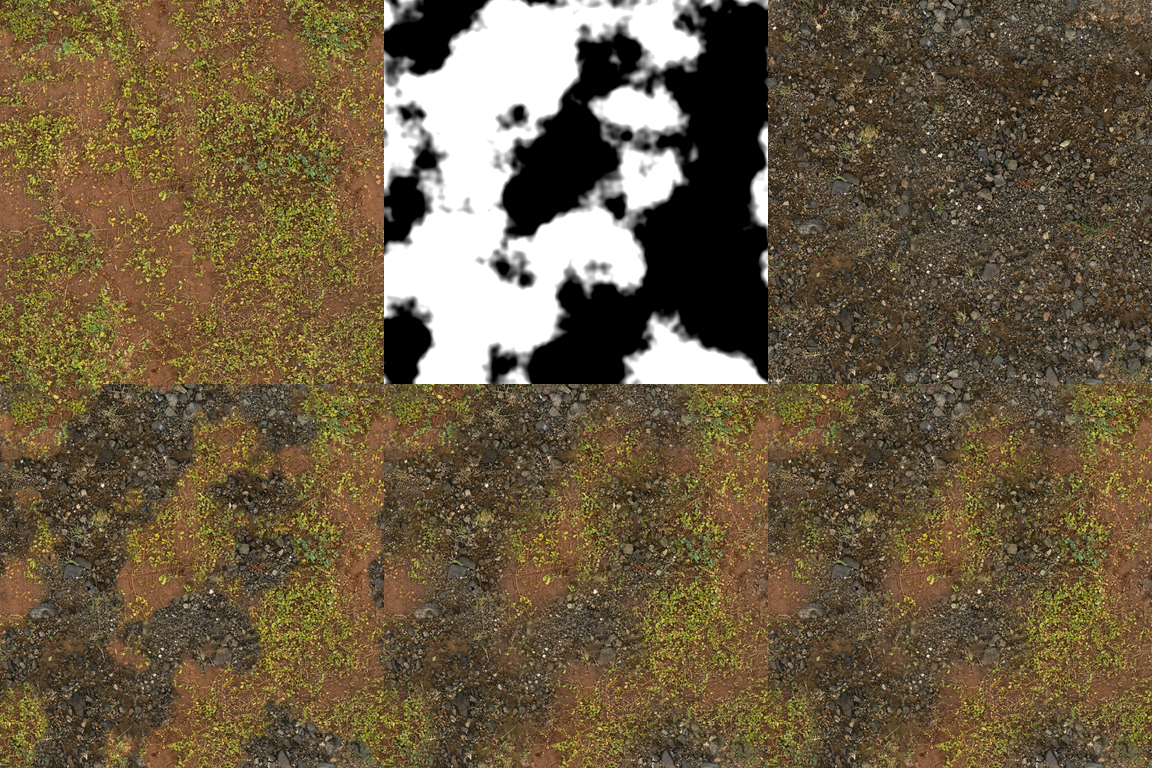
\includegraphics[width=0.89\linewidth]{materiais_perlin.png}
\caption{Par de materiais com máscara Perlin. Acima, textura A, máscara e textura B. Abaixo, lerp, Laplaciano completo e Laplaciano com salto 2.}
\label{fig:piloto}
\end{figure}

\section{Limitações e próximos passos}
Os resultados cobrem duas combinações de albedo de um único conjunto de ativos e uma implementação offline com reamostragem bilinear. A contagem analítica considera três amostras lógicas por nível para duas texturas e uma máscara. Ela passa de \(3(6+1)=21\) para \(3(3+1)=12\), redução de 42,9\%. Essa contagem depende do modelo de amostragem e não estima tempo de renderização, custo dos passes de máscara ou tráfego de memória.

Para concluir, vamos medir tempo por passe com consultas de tempo de GPU, usando resolução fixa, aquecimento e repetições. A avaliação visual será ampliada com materiais e máscaras adicionais, transições de diferentes larguras e recortes de artefatos. A seleção adaptativa por LOD e a comparação entre filtros podem ser avaliadas após o experimento principal.

\section{Conclusão preliminar}
Neste piloto, a omissão de níveis aproximou a mistura completa nos quatro cenários. A relação entre fidelidade visual e tempo de GPU ainda precisa ser medida antes de recomendar o método para renderização em tempo real.

\bibliographystyle{plain}
\bibliography{references}
\end{document}
